%%
%% Copyright 2026 Elsevier Ltd
%%
%% This file is part of the 'Elsarticle Bundle'.
%% ---------------------------------------------
%%
%% It may be distributed under the conditions of the LaTeX Project Public
%% License, either version 1.2 of this license or (at your option) any
%% later version.  The latest version of this license is in
%%    http://www.latex-project.org/lppl.txt
%% and version 1.2 or later is part of all distributions of LaTeX
%% version 1999/12/01 or later.
%%
%% The list of all files belonging to the 'Elsarticle Bundle' is
%% given in the file `manifest.txt'.
%%

%% Template article for Elsevier's document class `elsarticle'
%% with numbered style bibliographic references
%% SP 2008/03/01

\documentclass[preprint,12pt, a4paper]{elsarticle}

%% Use the option review to obtain double line spacing
%% \documentclass[authoryear,preprint,review,12pt]{elsarticle}

%% For including figures, graphicx.sty has been loaded in
%% elsarticle.cls. If you prefer to use the old commands
%% please give \usepackage{epsfig}

%% The amssymb package provides various useful mathematical symbols
\usepackage{amsmath}
\usepackage{amssymb}
\usepackage{amsfonts}
\usepackage{pifont}
\newcommand{\xmark}{\ding{55}}

%% Tables
\usepackage{booktabs}
\usepackage{tabularx}
\usepackage{array}
\usepackage{multirow}

%% Lists, links, listings
\usepackage{enumitem}
\usepackage{hyperref}
\usepackage{xcolor}
\usepackage{listings}
\usepackage{float}
\usepackage{caption}
\captionsetup[table]{skip=6pt} % space between table caption and table
%% ---- Revision markup (R1) ---------------------------------------------------
%% \showrevtrue  -> marked manuscript (revised text in blue)
%% \showrevfalse -> clean manuscript
\newif\ifshowrev
\showrevtrue
\ifshowrev
  \newcommand{\rev}[1]{{\color{blue}#1}}
\else
  \newcommand{\rev}[1]{#1}
\fi
\newcommand{\zl}[1]{{\textcolor{blue}{Check: #1}}}
\newcommand{\ab}[2]{{\textcolor{green}{Check: #1}}}

\setlength{\parindent}{0pt}
%% The amsthm package provides extended theorem environments
%% \usepackage{amsthm}

%% The lineno packages adds line numbers. Start line numbering with
%% \begin{linenumbers}, end it with \end{linenumbers}. Or switch it on
%% for the whole article with \linenumbers.
%\usepackage{lineno}

%% ---- Listings style (transferred from the IEEE source) ---------------------
\definecolor{backgroundColour}{HTML}{F8F8F8}
\definecolor{keywordclr}{HTML}{AA00FF}
\definecolor{commentclr}{HTML}{649696}
\definecolor{stringsclr}{HTML}{11A579}
\lstdefinestyle{PythonStyle}{
    language=Python,
    backgroundcolor=\color{backgroundColour},
    keywordstyle=\color{keywordclr},
    stringstyle=\color{stringsclr},
    commentstyle=\color{commentclr},
    upquote=true,
    basicstyle=\ttfamily\linespread{0.9}\footnotesize,
    breakatwhitespace=false,
    breaklines=true,
    captionpos=b,
    keepspaces=true,
    numbers=left,
    numbersep=5pt,
    numberstyle=\color{commentclr}\ttfamily\tiny,
    showspaces=false,
    showstringspaces=false,
    showtabs=false,
    tabsize=2,
    xleftmargin=2.25em,
    frame=single,
    framexleftmargin=1.25em,
    morekeywords={assert,with,as,None}
}
\lstset{style=PythonStyle}

\journal{SoftwareX}

\begin{document}

\begin{frontmatter}

%% Title, authors and addresses

%% use the tnoteref command within \title for footnotes;
%% use the tnotetext command for theassociated footnote;
%% use the fnref command within \author or \address for footnotes;
%% use the fntext command for theassociated footnote;
%% use the corref command within \author for corresponding author footnotes;
%% use the cortext command for theassociated footnote;
%% use the ead command for the email address,
%% and the form \ead[url] for the home page:

\title{\texttt{HiveWatch}: Framework-Agnostic Observability for Federated Learning}

%% use optional labels to link authors explicitly to addresses:

\author[anl,umass]{Abhijit Chunduru}
\ead{schunduru@anl.gov}

\author[anl]{Zilinghan Li}
\ead{zilinghan.li@anl.gov}

\author[anl]{Matthew Joel}
\ead{mjoel@anl.gov}

\author[anl,uchicago]{Ravi Madduri\corref{cor1}}
\ead{madduri@anl.gov}

\cortext[cor1]{Corresponding author}

\address[anl]{Argonne National Laboratory, Lemont, IL, USA}
\address[umass]{University of Massachusetts Amherst, Amherst, MA, USA}
\address[uchicago]{The University of Chicago, Chicago, IL, USA}

\begin{abstract}
%% Text of abstract
We present \texttt{HiveWatch}, an open-source, framework-agnostic observability toolkit for federated learning (FL). \texttt{HiveWatch} provides a minimal five-call training-lifecycle API and an FL-native schema for round summaries, client updates, communication volume, resource utilization, staleness measurements, failure events, and geographic metadata. A pluggable emitter interface routes a single normalized event stream simultaneously to replayable local JSONL artifacts and a geographic dashboard through \texttt{GeoEmitter}, Weights \& Biases through \texttt{WandbEmitter}, and MLflow through \texttt{MLflowEmitter}. We demonstrate \texttt{HiveWatch}'s portability across three architecturally distinct FL frameworks, APPFL, Flower, and NVIDIA FLARE, using the same API in each case. In a synthetic server-side microbenchmark of 50 rounds and 20 clients per round on an AWS EC2 \texttt{t3.medium} instance with 2 vCPUs and 4~GiB of RAM, internal bookkeeping required an average of 7.3$\mu$s per client-update call and 102.3$\mu$s per round-summary call, whereas the synchronous \texttt{GeoEmitter} required 3.02ms and 3.52ms, respectively. The software, framework integrations, examples, tests, and benchmark artifacts are available under the MIT License in the versioned \rev{v0.3.1} release.
\end{abstract}

\begin{keyword}
%% keywords here, in the form: keyword \sep keyword
Federated Learning \sep Observability \sep Experiment Tracking \sep MLflow \sep Weights and Biases \sep Map Visualization \sep Software

%% PACS codes here, in the form: \PACS code \sep code

%% MSC codes here, in the form: \MSC code \sep code
%% or \MSC[2008] code \sep code (2000 is the default)

\end{keyword}

\end{frontmatter}

%\linenumbers

\section*{Required Metadata}
\label{}
\section*{Current code version}
\label{}
\begin{table}[H]
\begin{tabular}{|l|p{4.5cm}|p{7.5cm}|}
\hline
\textbf{Nr.} & \textbf{Code metadata description} & \textbf{Please fill in this column} \\
\hline
C1 & Current code version & \rev{v0.3.1}\\
\hline
C2 & Permanent GitHub link to code/repository used for this code version & \rev{\url{https://github.com/APPFL/hivewatch/releases/tag/v0.3.1}}\\
\hline
C3 & Legal Code License   & MIT License \\
\hline
C4 & Code versioning system used & git \\
\hline
C5 & Software code languages, tools, and services used & Python\,$\geq$\,3.8; optional extras: \texttt{wandb}\,$\geq$\,0.16 (Weights \& Biases backend), \texttt{mlflow}\,$\geq$\,2.0 (MLflow backend), \texttt{requests}\,$\geq$\,2.25 (client geolocation helpers); no mandatory third-party dependencies for the core package \\
\hline
C6 & Compilation requirements, operating environments \& dependencies & \texttt{pip install hivewatch} from source or PyPI; Linux, macOS, Windows; no compilation step required; full dependency specification in \texttt{pyproject.toml} \\
\hline
C7 & If available Link to developer documentation/manual & \url{https://appfl.github.io/hivewatch}; runnable examples for APPFL, Flower, and NVIDIA FLARE in \texttt{examples/} at the repository root \\
\hline
C8 & Support email for questions & \{schunduru, zilinghan.li, mjoel, madduri\}@anl.gov \\
\hline
\end{tabular}
\caption{Code metadata (mandatory)}
\label{tab:codemeta}
\end{table}

% \zl{What is the difference between Table 1 and Table 4. \ab{table 4 can be omitted} We also need to remove the following paragraph before submitting, just noted to myself here.
% Ancillary data table required for subversion of the codebase. Kindly replace examples in right column with the correct information about your current code, and leave the left column as it is.
% @Abhijit: Please check the rules and policies, and remove this paragraph before you submit} \ab{sure}


\clearpage

% \textbf{Main text}\\

\section{Motivation and significance}
\label{sec:motivation}
Federated learning (FL) is a distributed machine learning paradigm that enables multiple clients to collaboratively train models without sharing raw data~\rev{\cite{mcmahan2017communication,zaland2025guarding}}, making it particularly valuable in privacy-sensitive domains such as healthcare~\cite{rieke2020future,hoang2025enabling}, finance~\cite{wang2019measure,wang2019interpret}, edge computing~\rev{\cite{lim2020federated,devaraj2024ruralai,que2025scalable}}\rev{, robotics~\cite{zaland2025federated}}, and multi-institutional research~\cite{kairouz2021advances,li2026scalable}. As FL deployments increase in scale and complexity, they present distinct {observability} challenges that existing tools do not adequately address. A single federated training run can involve many geographically distributed clients with heterogeneous data distributions, compute capabilities, communication costs, and failure modes~\rev{\cite{li2020federated,chen2024adaptive,chen2024robust}}. Without a unified monitoring layer, practitioners must manually consolidate fragmented logs, redefine client-level metric schemas for each new project \rev{ or framework, and are often limited to the monitoring backends supported by a particular framework}.

Several existing general-purpose experiment tracking tools, such as Weights \& Biases~\cite{wandb}, MLflow~\cite{mlflow}, and TensorBoard~\cite{tensorboard}, are designed primarily for centralized training. However, they lack native abstractions for federated rounds, client populations, per-client staleness, and client geography, all of which are important for monitoring in federated settings. Adapting these tools to FL typically requires devising a project-specific naming scheme for per-client metrics and recomputing derived quantities such as \rev{gradient-norm dispersion} and communication volume for each implementation. Modern FL frameworks, including APPFL~\cite{ryu2022appfl,li2025advances}, Flower~\cite{beutel2020flower}, and NVIDIA FLARE~\cite{roth2022nvidia}, provide their own logging facilities, \rev{ and some offer mature experiment-tracking support. For example, NVIDIA FLARE can stream client- and server-side metrics to TensorBoard, MLflow, and Weights \& Biases through its built-in tracking components, and FL platforms such as Fedstellar~\cite{beltran2024fedstellar} include their own monitoring dashboards. However, these facilities are specific to each runtime: metric names, the granularity of per-client records, and the FL-specific quantities captured differ across frameworks, and signals such as staleness, failures, and communication volume are largely left to the user to define.} Switching frameworks therefore requires practitioners to \rev{adapt their instrumentation and dashboards.} Another limitation lies in the gap between FL research and monitoring practice. Although prior research on heterogeneity and straggler management identifies important FL-specific metrics and diagnostics~\rev{\cite{chen2024adaptive,chen2024robust,xie2019asynchronous,nguyen2022federated,li2024fedcompass}}, existing tools do not provide a portable mechanism for collecting and visualizing these measurements consistently across FL frameworks.

\texttt{HiveWatch} addresses these limitations. It provides a framework-agnostic runtime API and an FL-native event schema, covering round starts, per-client updates, round summaries, failures, and checkpoints, that serve as an abstraction layer between an FL framework and one or more monitoring backends. The same instrumentation code can simultaneously stream experiment data to replayable local artifacts, Weights \& Biases, and MLflow, with derived metrics such as \rev{gradient-norm dispersion}, communication volume, and per-round wall time computed once within \texttt{HiveWatch} and forwarded to every configured backend. This design separates the \emph{what} of observability (the FL-specific schema) from the \emph{where} of observability (the choice of backend), so that practitioners can instrument once and monitor anywhere. \rev{Table~\ref{tab:comparison} summarizes how \texttt{HiveWatch} compares with existing experiment-tracking tools and the native monitoring facilities of FL frameworks.}

\begin{table}[t]
\caption{\rev{Comparison of \texttt{HiveWatch} with general-purpose experiment trackers and native monitoring facilities of FL frameworks. \checkmark: supported natively; $\circ$: partially supported or requires user-defined metrics; \xmark: not supported. For \texttt{HiveWatch}, staleness and communication statistics are computed from fields supplied by the framework adapter.}}
\label{tab:comparison}
\centering
\scriptsize
\ifshowrev\color{blue}\fi
\setlength{\tabcolsep}{3pt}
\begin{tabular}{lcccccc}
\toprule
\textbf{Tool} & \textbf{\shortstack{Framework\\independent}} & \textbf{\shortstack{FL-native\\schema}} & \textbf{Staleness} & \textbf{\shortstack{Failure\\tracking}} & \textbf{\shortstack{Comm.\\statistics}} & \textbf{\shortstack{Multi-\\backend}} \\
\midrule
W\&B/MLflow/TensorBoard & \checkmark & \xmark & \xmark & \xmark & \xmark & \xmark \\
APPFL & \xmark & $\circ$ & $\circ$ & \xmark & $\circ$ & \xmark \\
Flower & \xmark & $\circ$ & \xmark & $\circ$ & \xmark & \xmark \\
NVIDIA FLARE & \xmark & $\circ$ & \xmark & \xmark & \xmark & \checkmark \\
Fedstellar & \xmark & \checkmark & \xmark & $\circ$ & $\circ$ & \xmark \\
\texttt{HiveWatch} (this work) & \checkmark & \checkmark & \checkmark & \checkmark & \checkmark & \checkmark \\
\bottomrule
\end{tabular}
\end{table}


\section{Software description}
\label{sec:software}

\subsection{Software Architecture}

\begin{figure*}[!htbp]
    \centering
    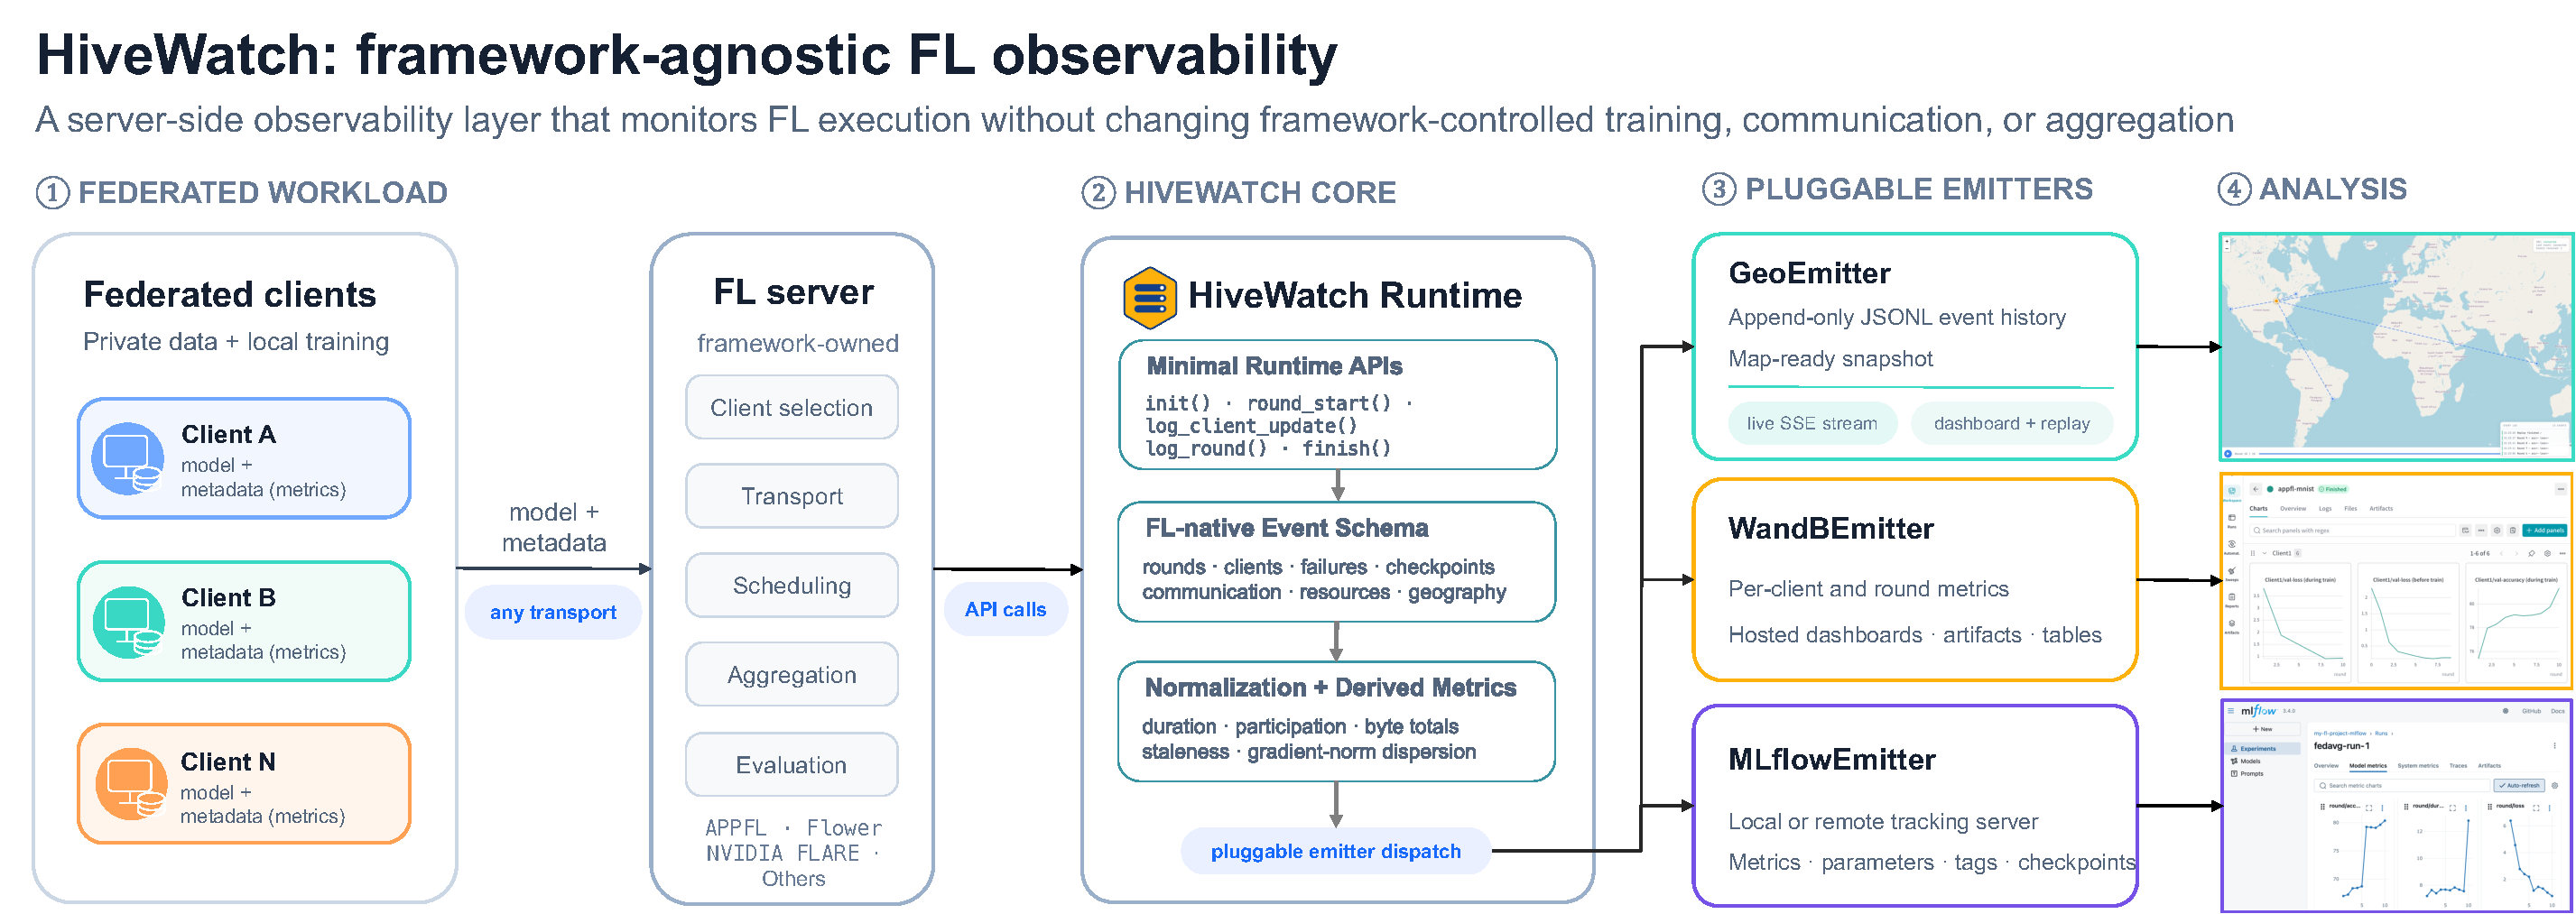
\includegraphics[width=\linewidth]{images/arch.pdf}
    \caption{Architecture of \texttt{HiveWatch}, a framework-agnostic observability layer for FL. Federated clients transmit models and training metadata to a framework-managed FL server through any supported transport. The server invokes the minimal \texttt{HiveWatch} runtime APIs, which represent execution activity using an FL-native event schema and compute normalized and derived metrics. A pluggable dispatcher then forwards the resulting records concurrently to the geographic, Weights \& Biases, and MLflow emitters for visualization, experiment tracking, and replay without modifying framework-controlled training, communication, or aggregation.}
    \label{fig:hivewatch}
\end{figure*}

As illustrated in Figure~\ref{fig:hivewatch}, \texttt{HiveWatch} is a framework-agnostic, server-side observability layer that connects an existing federated learning framework to one or multiple monitoring backends. The FL framework remains fully responsible for client selection, model distribution, local training, communication, evaluation, and model aggregation. At selected points in the server-side control flow, the framework invokes \texttt{HiveWatch}'s minimal runtime APIs to record FL-native events. \texttt{HiveWatch} normalizes these events, computes derived metrics, and dispatches the resulting records to all configured emitters without modifying the underlying communication protocol or aggregation algorithm. This decouples FL-specific observability from both the training framework and monitoring backend, enabling effortless integration with architecturally distinct frameworks such as APPFL, Flower, NVIDIA FLARE, and custom training loops through the same runtime interface.



\subsection{Software Functionalities}

\begin{table}[H]
\caption{\texttt{HiveWatch} runtime APIs.}
\label{tab:api}
\centering
\footnotesize
\begin{tabular}{ll}
\toprule
\textbf{Call} & \textbf{When to invoke} \\
\midrule
\texttt{hivewatch.init(\ldots)}
    & Once at server startup \\
\texttt{hivewatch.round\_start(round)}
    & At the start of each global round \\
\texttt{hivewatch.log\_client\_update(id, **kwargs)}
    & When a client update is received \\
\texttt{hivewatch.log\_round(round, \ldots)}
    & After each aggregation round \\
\texttt{hivewatch.finish()}
    & Once at server shutdown \\
\bottomrule
\end{tabular}
\end{table}


\textbf{Runtime APIs.}
\texttt{HiveWatch} exposes five primary runtime calls, as summarized in Table~\ref{tab:api}. At server startup, \texttt{init()} initializes the monitoring run and its configured emitters. During each training round, the server 
records the round start (\texttt{round\_start()}), logs each client update as it arrives (\texttt{log\_client\_update()}), and emits the final round-level summary after aggregation (\texttt{log\_round()}). Finally, \texttt{finish()} finalizes the run and closes the configured emitters. These calls correspond to common stages of the server-side FL lifecycle, allowing \texttt{HiveWatch} to instrument different FL frameworks and custom training loops through a consistent interface.

\textbf{Event Schema.}
The FL-native event schema represents monitoring information at both the client and round levels. Client update events may include local accuracy, local loss, sample count, gradient norm and sparsity, bytes sent and received, training wall time, CPU, RAM and GPU utilization, geographic metadata (\texttt{lat}/\texttt{lng}/\texttt{country}), and asynchronous staleness, represented by the originating model round (\texttt{base\_round}). Unrecognized framework-specific fields are preserved verbatim, allowing frameworks to extend the standard schema without modifying \texttt{HiveWatch}. Round summary events record global accuracy and loss, per-round wall time, the number of clients selected and the number that completed training, straggler and failure counts, total communication volume, \rev{gradient-norm dispersion,} defined as the standard deviation of per-client gradient norms, and aggregation time. \rev{Specifically, gradient-norm dispersion is a lightweight, magnitude-only indicator of client-update heterogeneity: it only requires per-client scalar norms, but it does not capture differences in gradient direction, which would require processing the full update vectors on the server's critical path.} Derived quantities are computed once within \texttt{HiveWatch} and forwarded to every configured emitter backend.

\begin{figure*}[t]
\centering
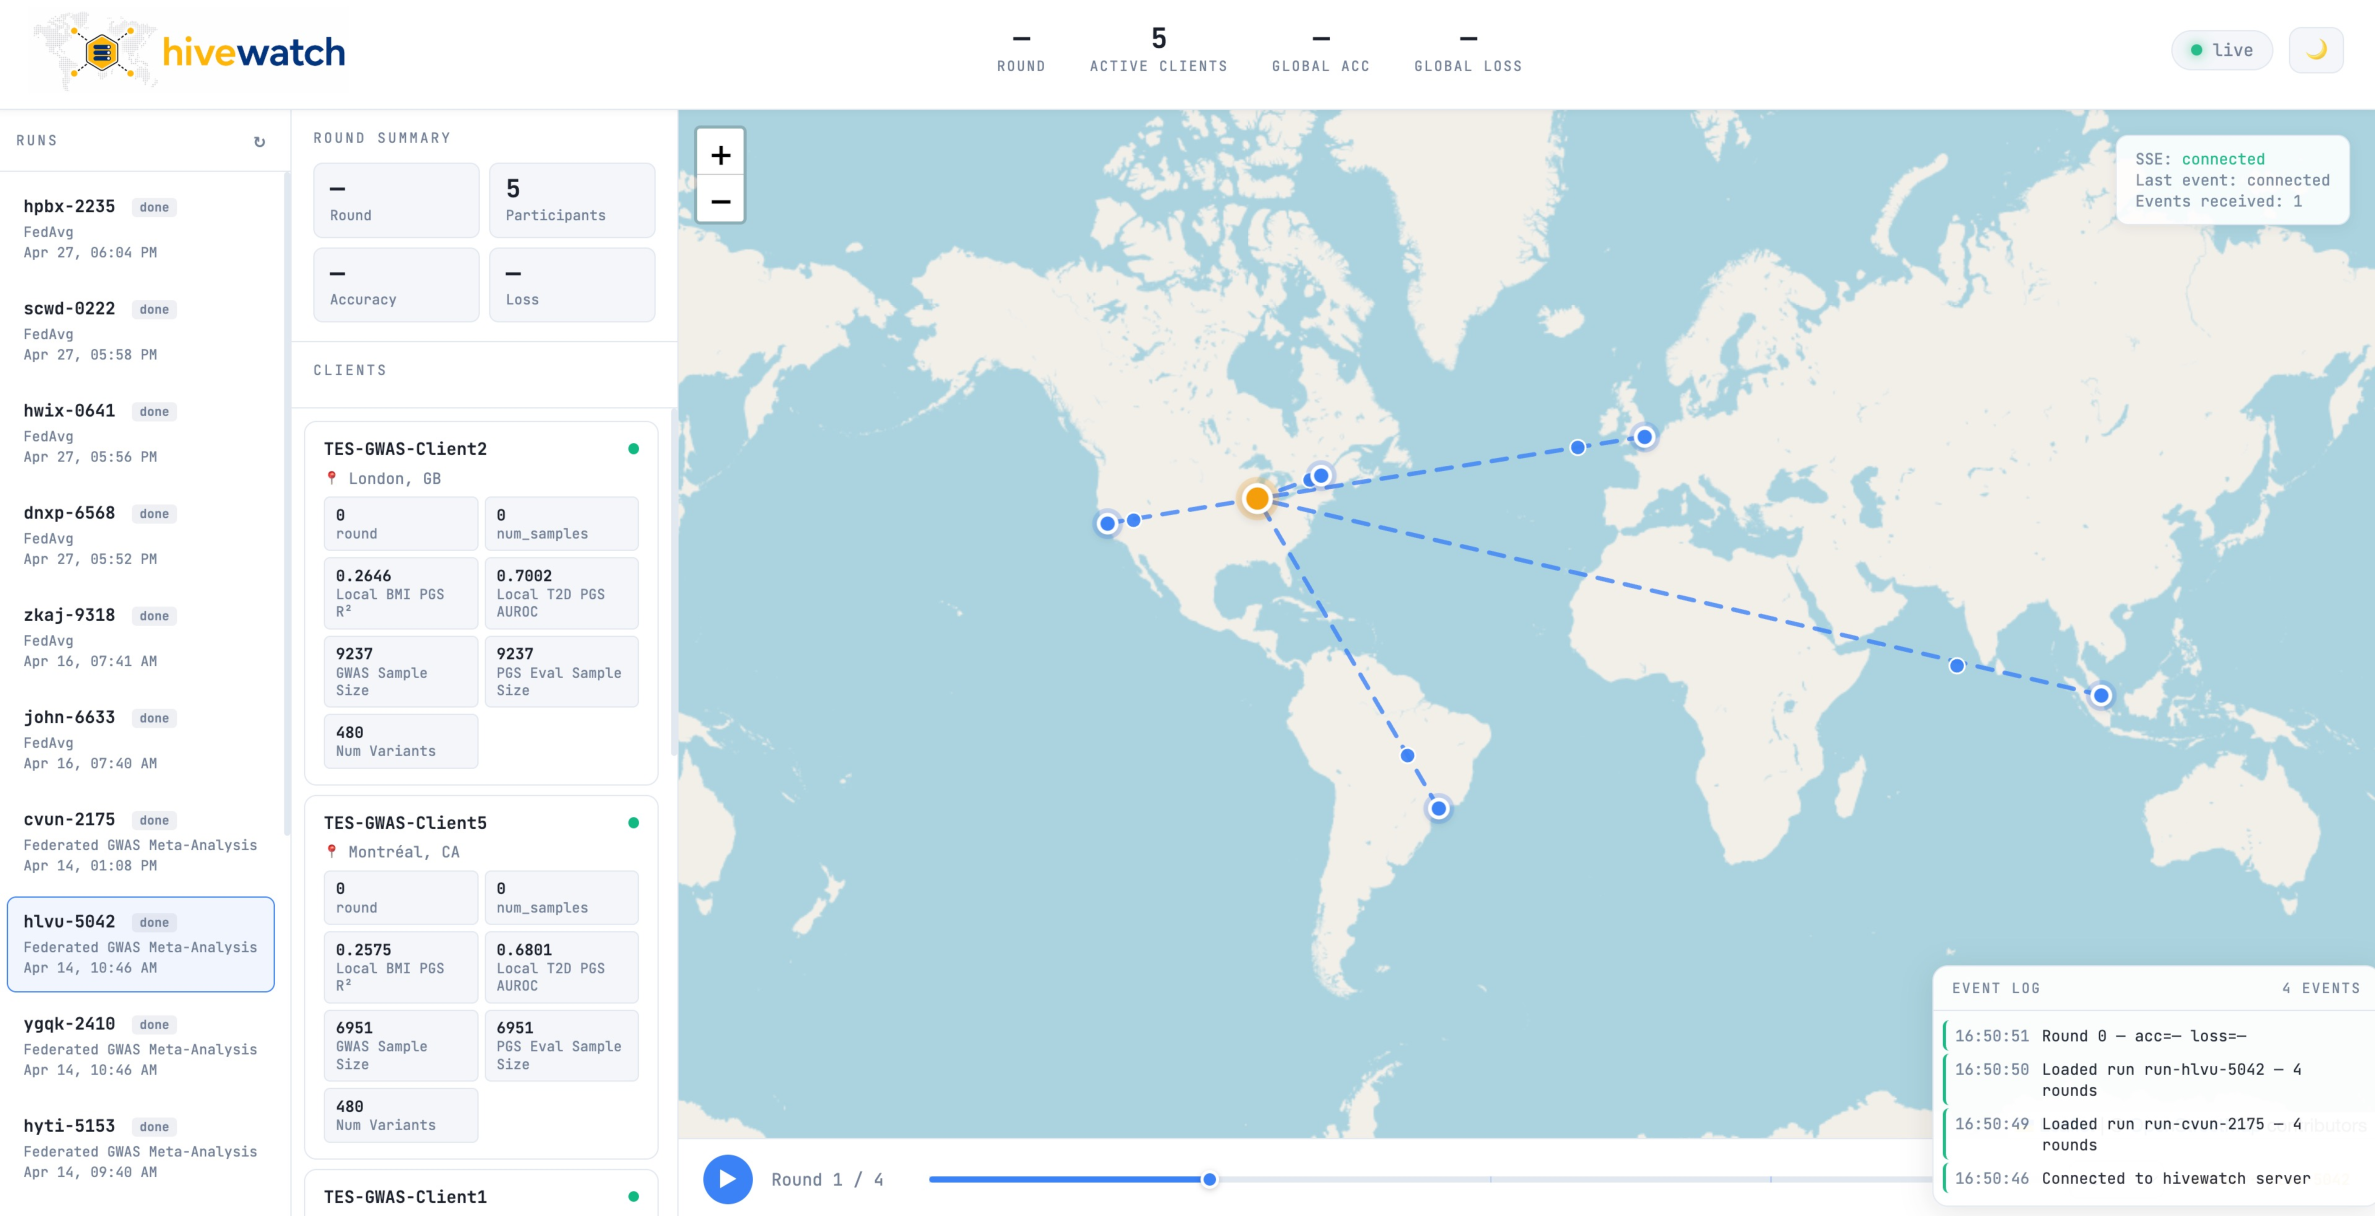
\includegraphics[width=\textwidth]{images/example.pdf}
\caption[HiveWatch map dashboard for a federated GWAS experiment.]
{Example of the \texttt{HiveWatch} map dashboard used to monitor a federated GWAS meta-analysis across five geographically distributed GA4GH TES endpoints~\cite{chunduru2026towards}. The map visualizes the connections between the aggregation server and participating clients, while the side panels display run-level and client-level metadata and the timeline supports round-by-round replay.}
\label{fig:example}
\end{figure*}
\textbf{Emitter Backends.}
\texttt{HiveWatch} decouples metric collection and processing from metric storage and visualization through a pluggable emitter interface. Multiple emitters can be configured concurrently, allowing the same event stream to be delivered to complementary monitoring systems. \texttt{HiveWatch} currently implements the following three emitters:

\begin{itemize}[noitemsep]
    \item \textbf{GeoEmitter:} For each event, appends a record to a replayable JSONL event log and updates a map-ready \texttt{.map.json} snapshot. Because the event history is append-only and persisted incrementally, the artifacts remain available if the monitoring or training process terminates unexpectedly and can be used for post-hoc analysis without re-running training.
    \item \textbf{WandbEmitter:} Logs per-client and per-round metrics to Weights \& Biases, using \texttt{wandb.define\_metric()} to align all metric series with the round axis.
    \item \textbf{MLflowEmitter:} Records metrics, parameters, tags, and model checkpoint artifacts in a local or remote MLflow tracking server. Per-client metric names use dot notation to comply with MLflow's naming conventions.
\end{itemize}

Users can add custom emitters by implementing four callback methods: \texttt{on\_init}, \texttt{on\_round}, \texttt{on\_client\_update}, and \texttt{finish}. This interface enables additional storage, visualization, or alerting systems to consume the same normalized event stream without changing the \texttt{HiveWatch} runtime.

\textbf{Map Dashboard.}
The artifacts produced by \texttt{GeoEmitter} can be served and visualized on a map by the bundled \texttt{hivewatch map run} CLI, which launches a local browser-based dashboard showing client locations, training status, round progress, straggler markers, and per-client metadata. For active runs, the dashboard receives updates through server-sent events; for completed runs, it reconstructs the monitored execution from the saved artifacts. The same interface therefore supports both live monitoring and post-hoc replay. Figure~\ref{fig:example} shows the \texttt{HiveWatch} map dashboard for a federated GWAS meta-analysis conducted across geographically distributed GA4GH TES endpoints~\cite{chunduru2026towards}.


\subsection{Implementation Notes}

\texttt{HiveWatch} is a pure-Python package that supports Python~3.8 and later and is distributed  under the MIT License. The core package depends only on the Python standard library, which minimizes installation overhead and facilitates deployment in heterogeneous computing environments. Integrations with Weights \& Biases and MLflow, along with the optional client geolocation helper used by the map dashboard, can be installed as extras via \texttt{pip install hivewatch[wandb]}, \texttt{[mlflow]}, \texttt{[geo]}, or \texttt{[all]}. Internal state is protected by a single \texttt{threading.Lock}, making \rev{all runtime calls} safe to call across concurrent server threads. \rev{A failing emitter call during training is logged and skipped without interrupting training or the other configured emitters, whereas errors during emitter initialization are raised immediately.} The package distributes the map dashboard as a static HTML package-data asset, eliminating the need for a separate build process, JavaScript toolchain, or web bundler at installation time.


\section{Illustrative examples}
\label{sec:illustrative}

\subsection{Installation and Quickstart}

\texttt{HiveWatch} can be installed from PyPI via a single command:

\begin{lstlisting}[style=PythonStyle,language=bash,caption={Installation command for \texttt{HiveWatch}.}]
pip install hivewatch  # core only, no third-party deps
pip install hivewatch[all] # with W&B, MLflow, geolocation
\end{lstlisting}

The following listing illustrates the minimal instrumentation required to integrate \texttt{HiveWatch} into a framework-agnostic FL server loop using the \texttt{WandbEmitter} and \texttt{GeoEmitter}. Comments distinguish framework-managed training operations from \texttt{HiveWatch} monitoring calls.

\begin{lstlisting}[style=PythonStyle,caption={Minimal \texttt{HiveWatch} integration into an FL server loop.}]
import hivewatch
from hivewatch.emitters import GeoEmitter, WandbEmitter

hivewatch.init(
    algorithm="FedAvg",
    emitters=[
        GeoEmitter(runs_dir="runs", port=7070),
        WandbEmitter(project="my-fl-project"),
    ],
)

for round_num in range(num_rounds):
    hivewatch.round_start(round_num)

    # Clients perform local training and collect results
    # [FL-framework-specific-training-logic...]
    
    for client_id, result in client_results.items():
        hivewatch.log_client_update(
            client_id,
            round=round_num,
            local_accuracy=result["acc"],
            local_loss=result["loss"],
            num_samples=result["n"],
            bytes_sent=result["bytes"],
            train_time_sec=result["t"],
        )

    # Server aggregates client updates
    # [FL-framework-specific-aggregation-logic...]

    hivewatch.log_round(
        round_num,
        global_accuracy=agg_acc,
        global_loss=agg_loss,
    )

hivewatch.finish()
\end{lstlisting}

\subsection{Framework Integration}

We demonstrate \texttt{HiveWatch}'s framework-agnostic design and portability by integrating the same core runtime APIs with three popular FL frameworks that differ substantially in their architectures, client-server interaction patterns, and communication stacks. Full runnable examples are included in the \texttt{HiveWatch} source distribution's \texttt{example} folder.

\textbf{APPFL.} The APPFL integration subclasses APPFL's \texttt{ServerAgent} and overrides its \texttt{global\_update()} method, which processes incoming client updates. The integration invokes \texttt{round\_start()} on each round transition and \texttt{log\_client\_update()} after APPFL processes the corresponding update. All \texttt{HiveWatch} runtime calls remain on the server side.

\textbf{Flower.} The Flower integration subclasses Flower’s \texttt{FedAvg}.
Within the function \texttt{aggregate\_fit()}, it forwards per-client metrics carried in Flower's \texttt{FitRes} objects to \texttt{log\_client\_update()} and, within \texttt{aggregate\_evaluate()}, it records the round-level summary after the global metrics become available. Client failures reported through Flower's native interface are captured using the \texttt{log\_dropout()} function, one of several optional auxiliary runtime calls that complement the five core APIs listed in Table~\ref{tab:api}.

\textbf{NVIDIA FLARE.} The NVIDIA FLARE integration subclasses the framework's \texttt{FedAvg} controller to inject \texttt{HiveWatch} API calls into \texttt{send\_model()}, \texttt{\_aggregate\_one\_result()}, and \texttt{\_get\_aggregated\_result()}. It then registers the wrapped controller in the recipe's deployment map.

The framework-specific adapter is confined to a single server-side file for each framework, with approximately 75 added lines of code for APPFL and Flower, and 115 lines for NVIDIA FLARE. The larger NVIDIA FLARE adapter reflects the additional steps required to reconstruct the controller and replace it in the deployment map. None of the three integrations requires modifications to the core \texttt{HiveWatch} implementation itself.

Client implementations remain framework-native and generally require no \texttt{HiveWatch} instrumentation. The Flower example uses no \texttt{HiveWatch} calls on the client; instead, each client populates Flower's native \texttt{fit()} metrics dictionary, which the server-side adapter then forwards to \texttt{HiveWatch}. The only optional client-side addition is a call to \texttt{HiveWatch}'s \texttt{get\_location()} helper function when geographic metadata is needed for visualization in the map dashboard. The APPFL and NVIDIA FLARE examples use this helper to tag each update with the client's geographic coordinates.

\subsection{Instrumentation Overhead}

As \texttt{HiveWatch} executes on the server's critical path, its overhead should remain small relative to the duration of an FL round. We benchmark the two primary data-recording calls reported in Table~\ref{tab:overhead}, \texttt{log\_client\_update()} and \texttt{log\_round()}, using 50 FL global rounds with 20 clients per round. Each trial therefore contains 1{,}000 client-update calls and 50 round-summary calls, with 1{,}050 measured calls in total. We compare two configurations: no emitter, which isolates in-memory bookkeeping, and \texttt{GeoEmitter}, which adds a synchronous JSONL append and a complete rewrite of the \texttt{.map.json} snapshot for each event. The workload for this microbenchmark is synthetic, with no model, dataset, or FL framework involved; therefore, the reported times isolate instrumentation overhead from FL-related workflow costs including training, communication, and aggregation.

To assess repeatability, we execute five independent trials. Table~\ref{tab:overhead} reports descriptive statistics pooled across the resulting 5{,}000 \texttt{log\_client\_update()} calls and 250 \texttt{log\_round()} calls. For each call--configuration pair, the value following $\pm$ is the standard deviation across all pooled calls, whereas the final column reports the standard deviation of the mean values of the five independent trials. The measurement script is included in the repository as \texttt{benchmarks/instrumentation\_overhead.py}, and the script to aggregate the repeated trials is available at \texttt{benchmarks/aggregate\_overhead.py}. Together, these scripts allow the benchmark procedure to be reproduced on other systems, although the absolute measurements will depend on the underlying hardware and software environment.

All measurements from Table~\ref{tab:overhead} were collected on an AWS EC2 \texttt{t3.medium} instance (2 vCPUs, Intel Xeon Platinum 8259CL @ 2.50GHz, 4~GiB RAM) running Ubuntu 26.04 LTS with Python 3.14.4. The \texttt{GeoEmitter} JSONL and \texttt{.map.json} artifacts were written to an EBS SSD root volume exposed through the NVMe interface.\footnote{\texttt{t3.medium} is a burstable, shared-resource instance type; absolute latencies may differ with available CPU credits, host contention, storage configuration, and the use of dedicated-core hardware.} 

\begin{table}[t]
\caption{Per-call instrumentation overhead ($\mu$s), pooled over 5 independent trials of 50 rounds $\times$ 20 clients each. The p95 value is the 95th-percentile latency, meaning that 95\% of observed calls completed at or below the reported value. The trial-level standard deviation is computed over the five trial-level means.}
\label{tab:overhead}
\scriptsize
\centering
\begin{tabular}{lrrrr}
\toprule
\textbf{Call (configuration)} & \textbf{\shortstack{Mean$\pm$Call-level Std}} & \textbf{Median} & \textbf{p95} & \textbf{\shortstack{Trial-level Std}} \\
\midrule
\texttt{log\_client\_update} (no emitter) & 7.3$\pm$1.9 & 6.7 & 9.8 & 0.1 \\
\texttt{log\_round} (no emitter)           & 102.3$\pm$26.3 & 93.4 & 155.4 & 3.6 \\
\texttt{log\_client\_update} (\texttt{GeoEmitter})  & 3{,}024.7$\pm$1{,}935.2 & 2{,}929.2 & 5{,}653.5 & 192.3 \\
\texttt{log\_round} (\texttt{GeoEmitter})           & 3{,}518.8$\pm$1{,}916.5 & 3{,}472.8 & 6{,}025.2 & 166.1 \\
\bottomrule
\end{tabular}
\end{table}

Without an emitter, the mean overhead is 7.3$\mu$s for \texttt{log\_client\_update()} and 102.3$\mu$s for \texttt{log\_round()}. These measurements capture schema normalization, derived-metric computation, and round-state bookkeeping. The \texttt{GeoEmitter} raises the mean overhead to approximately 3.0-3.5ms. This increase is primarily associated with synchronously persisting each JSONL event and rewriting the map metadata snapshot. The synchronous design favors artifact consistency and recoverability: events persisted before a failure remain available for post-hoc replay.

Summed over a 20-client round, the \texttt{GeoEmitter} adds approximately 64ms of server-side overhead across 20 client-update calls and one round-summary call, which is negligible relative to real FL round durations (usually takes at least seconds to minutes). Across all four call--configuration pairs, the standard deviation of the five trial-level means (0.1--192.3$\mu$s) was substantially smaller than the corresponding pooled call-level standard deviation (1.9--1{,}935.2$\mu$s). This difference indicates that the observed latency variation arose primarily among individual calls within each trial, while the average performance remained relatively stable across independent trials.

We only benchmark the \texttt{GeoEmitter} in the experiments because it is the bundled persistence backend whose synchronous, local storage path can be measured reproducibly without dependence on an external service. \texttt{WandbEmitter} and \texttt{MLflowEmitter} are excluded because they rely on external monitoring tools and their observed latency depends on factors such as SDK operating mode, local buffering, batching, network conditions, tracking-server location, and backend load. A single measurement would therefore be difficult to reproduce or interpret across deployments. These emitters may still incur serialization, buffering, networking, or local-persistence costs, and the results in Table~\ref{tab:overhead} should not be interpreted as latency bounds for either integration. \rev{Qualitatively, \texttt{MLflowEmitter} issues at least one synchronous \texttt{log\_batch} request per event, so its per-call latency is dominated by the round trip to the tracking server, whereas \texttt{WandbEmitter} hands records to the W\&B SDK, which uploads them asynchronously from a background process by default. We likewise do not compare against the native logging of each framework, since these record different metric sets and are therefore not like-for-like baselines.}

% \zl{
%  Run-to-run standard deviation of the trial means --- i.e.
% variation between the 5 independent process repetitions rather than
% within-run call-to-call jitter --- was small (0.1--192\,$\mu$s across
% configurations), indicating the pooled standard deviation above is
% dominated by per-call jitter rather than systematic drift between runs.
% The \texttt{WandbEmitter} and \texttt{MLflowEmitter} offload persistence to
% external services and do not incur per-call file I/O.
% }


\section{Impact}
\label{sec:impact}
\texttt{HiveWatch} addresses three FL practitioner needs that are not adequately supported by existing tools.

\textbf{Portable instrumentation across FL frameworks.} Researchers who work with multiple FL frameworks or who plan to migrate from one to another currently must maintain framework-specific instrumentation and metric conventions. \texttt{HiveWatch} provides a single FL-native runtime interface and event schema that can be easily reused across APPFL, Flower, NVIDIA FLARE, and custom training loops. Although each framework requires a lightweight server-side adapter, the monitoring logic remains expressed through the same five core runtime calls and does not need to be reimplemented for each backend. \rev{\texttt{HiveWatch} complements, rather than replaces, native tracking facilities such as those of NVIDIA FLARE and APPFL: its contribution is a common FL-native schema and derived metrics that remain consistent when the framework changes.}

\textbf{Simultaneous multi-backend monitoring.} Teams frequently need to send experiment records to more than one destination, such as local artifacts for immediate debugging and replay, a hosted dashboard for cross-run comparison, and a self-hosted tracking server for compliance or reproducibility. \texttt{HiveWatch}'s emitter model fans out the same normalized event stream to multiple configured backends without duplicating framework instrumentation. In addition, the \texttt{GeoEmitter}'s replayable JSONL artifacts allow completed or interrupted runs to be inspected offline without re-running training.

\textbf{FL-native diagnostics.} \texttt{HiveWatch}'s schema captures straggler counts, \rev{gradient-norm dispersion} as an indicator of client-update heterogeneity, per-client staleness in asynchronous FL, communication volume breakdowns, client dropout and failure events, and optional geographic client metadata. General-purpose tracking tools such as Weights \& Biases or MLflow can store such values, but they do not provide native FL abstractions or automatically derive them from a common event schema; practitioners must instead define project-specific metrics and instrumentation logic. Collectively, these signals expose the system and statistical conditions addressed by client-selection, heterogeneity-mitigation, and asynchronous-aggregation methods~\cite{chen2024adaptive,xie2019asynchronous,li2024fedcompass,lai2021oort,chen2023exploring}. Logging them consistently enables practitioners to characterize heterogeneity and failure behavior, compare these effects across deployments, and evaluate which mitigation strategies are appropriate.

The primary audience of \texttt{HiveWatch} is FL practitioners and researchers who need reproducible, inspectable experiment records across diverse FL deployments, including multi-institutional biomedical FL, edge FL, and academic FL benchmarking. \texttt{HiveWatch} is released under the MIT license and developed openly at \url{https://github.com/APPFL/hivewatch} with documentation at \url{https://appfl.github.io/hivewatch}. The package is distributed through PyPI and can be installed with \texttt{pip install hivewatch}.

\section{Conclusions}
\label{sec:conclusion}
We presented \texttt{HiveWatch}, a lightweight, framework-agnostic observability layer for federated learning. By defining an FL-native event schema and decoupling metric collection from metric storage through a pluggable emitter interface, \texttt{HiveWatch} allows a common set of server-side instrumentation calls to deliver the same normalized event stream simultaneously to local replayable JSONL artifacts, Weights \& Biases, and MLflow. We demonstrated the portability of the design by integrating \texttt{HiveWatch} with APPFL, Flower, and NVIDIA FLARE using the same server-side APIs. At the evaluated scale, our microbenchmark measured mean per-call overheads of 7.3--102.3$\mu$s for internal bookkeeping and approximately 3.0--3.5ms when using the disk-persisting \texttt{GeoEmitter}. For a round involving 20 client updates, the measured \texttt{GeoEmitter} calls added approximately 64ms of server-side overhead, which is negligible for the time-scale of an FL round.

Current limitations include the use of a single-host map server intended for local debugging rather than production multi-user dashboard deployment; the requirement that applications map framework-specific result fields to \texttt{HiveWatch}'s schema within the bridging layer; and the synchronous rewriting of the map snapshot, whose cost may increase with snapshot size. Future work will investigate scalable dashboard deployment, incremental or asynchronous snapshot persistence, additional emitters (for systems such as Prometheus and TensorBoard), lightweight anomaly detection based on changes in gradient statistics and communication performance, and cross-run comparison views in the map dashboard.

%% ---- Declarations ----------------------------------------------------------
% ---- CRediT Author Contribution Statement ----------------------------------
\section*{CRediT Author Contribution Statement}
\textbf{Abhijit Chunduru:} Conceptualization, Software, Validation, Writing -- original draft, Writing -- review and editing.
\textbf{Zilinghan Li:} Conceptualization, Software, Validation, Writing -- original draft, Writing -- review and editing.
\textbf{Matthew Joel:} Software, Validation, Writing -- review and editing.
\textbf{Ravi Madduri:} Supervision, Funding acquisition, Writing -- review and editing.

% ---- Data Availability ------------------------------------------------------
\section*{Data Availability}
\texttt{HiveWatch} does not process or distribute datasets. The software source code, runnable examples, benchmark results, and documentation are publicly available at \url{https://github.com/APPFL/hivewatch} under the MIT License. No experimental datasets were used in producing the results in this paper; the instrumentation overhead figures were obtained by running the bundled \texttt{HiveWatch} package in a synthetic microbenchmark with no external data.

% ---- Declaration of Competing Interests -------------------------------------
\section*{Declaration of Competing Interests}
The authors declare that they have no known competing financial interests or personal relationships that could have appeared to influence the work reported in this paper.

% ---- Declaration of Generative AI ------------------------------------------
\section*{Declaration of Generative AI and AI-Assisted Technologies}
During the preparation of this work, the authors used Anthropic Claude and OpenAI ChatGPT to support language editing and manuscript drafting. The authors reviewed, verified, and edited all outputs and take full responsibility for the content of the published article.

\section*{Acknowledgements}
\label{}
This material is based upon work supported by the U.S.\ Department of Energy, Office of Science, under contract number DE-AC02-06CH11357. We also gratefully acknowledge Amazon Web Services for providing cloud computing credits that supported the experimental work for this manuscript.

%% The Appendices part is started with the command \appendix;
%% appendix sections are then done as normal sections
%% \appendix

%% \section{}
%% \label{}

%% References:
%% If you have bibdatabase file and want bibtex to generate the
%% bibitems, please use

\bibliographystyle{elsarticle-num}
\bibliography{references}

% \newpage
% \section*{Current executable software version}
% \label{}

% \begin{table}[!h]
% \begin{tabular}{|l|p{4.5cm}|p{7.5cm}|}
% \hline
% \textbf{Nr.} & \textbf{(Executable) software metadata description} & \textbf{Please fill in this column} \\
% \hline
% S1 & Current software version & v0.3.0 \\
% \hline
% S2 & Permanent link to executables of this version & \url{https://github.com/APPFL/hivewatch/releases/tag/v0.3.0}; installable via \texttt{pip install hivewatch}  \\
% \hline
% S3 & Legal Software License & MIT License \\
% \hline
% S4 & Computing platforms/Operating Systems & Linux, macOS, Windows (Python\,$\geq$\,3.8) \\
% \hline
% S5 & Installation requirements \& dependencies & \texttt{pip install hivewatch}; optional extras: \texttt{wandb\,$\geq$\,0.16}, \texttt{mlflow\,$\geq$\,2.0}, \texttt{requests}\,$\geq$\,2.25  \\
% \hline
% S6 & If available, link to user manual & \url{https://appfl.github.io/hivewatch};\\
% \hline
% S7 & Support email for questions & \{schunduru, zilinghan.li, mjoel, madduri\}@anl.gov \\
% \hline
% \end{tabular}
% \caption{Software metadata}
% \label{tab:softwaremeta}
% \end{table}

\end{document}
\endinput
%%
%% End of file `SoftwareX_article_template.tex'.
